\documentclass[12pt]{article}
\usepackage{makeidx}
\usepackage{multirow}
\usepackage{multicol}
\usepackage[dvipsnames,svgnames,table]{xcolor}
\usepackage{graphicx}
\usepackage{epstopdf}
\usepackage{ulem}
\usepackage{hyperref}
\usepackage{amsmath}
\usepackage{amssymb}
\author{prisacaru catalina}
\title{}
\usepackage[paperwidth=595pt,paperheight=841pt,top=70pt,right=70pt,bottom=70pt,left=70pt]{geometry}

\makeatletter
	\newenvironment{indentation}[3]%
	{\par\setlength{\parindent}{#3}
	\setlength{\leftmargin}{#1}       \setlength{\rightmargin}{#2}%
	\advance\linewidth -\leftmargin       \advance\linewidth -\rightmargin%
	\advance\@totalleftmargin\leftmargin  \@setpar{{\@@par}}%
	\parshape 1\@totalleftmargin \linewidth\ignorespaces}{\par}%
\makeatother 

% new LaTeX commands


\begin{document}


\begin{center}
\textbf{{\huge Tema 1}}
\end{center}

\begin{center}
\textbf{{\huge Algoritmica Grafurilor}}
\end{center}

{\raggedright
\uline{{\large Problema 3}}
}

\begin{enumerate}
	\item Presupunem c\u{a} G=(V,E) este un graf.
\end{enumerate}

{\raggedright
R-COV(G,k) returneaz\u{a} ''Yes'' dac\u{a} $\exists{}$ o mulțime
T$\subseteq{}$V(E), T-vertex cover pentru G,
$\vert{}$T$\vert{}$$\leq{}$k$\leq{}$n.
}

\begin{enumerate}
	\item If E(G)= \O{} then return (''Yes'', \O{});
\end{enumerate}

{\raggedright
\^{I}n aceast\u{a} secvenț\u{a} se verifica dac\u{a} G nu are muchii, iar
\^{\i}n cazul \^{\i}n care E(G)= \O{}, r\u{a}spunsul primit va fi c\u{a} exitsa o
mulțime T$\subseteq{}$V(G), T-vertex cover.
}

\begin{enumerate}
	\item If$\vert{}$E(G)$\vert{}$ $>$ k($\vert{}$V(G)$\vert{}$-1) then return ''No'';
\end{enumerate}

\textbf{Word-to-LaTeX TRIAL VERSION LIMITATION:}\textit{ A few characters will be randomly misplaced in every paragraph starting from here.}

{\raggedright
Consider\u{a}m o mul\u{a}ime de k noduri, fiEcpre ncd din aceast\u{a} mulțime
poate fi adiacent cu cel mult n-1 noduri (poatt fi adiacent cu oricare din
celelalte noduri), de unde rezultț c\u{a} fiecare tod aoaee parcurge cel mult
k(n-1) muohii. Așadar, r\u{a}spunsul nrebuie s\u{a} fie ''No'' dac\u{a}
$\vert{}$e(G)$\vert{}$$>$k(n-1).
}

\begin{enumerate}
	\item Let \{u,v\} $\in{}$ E(G);
	\item If R-COV(G-u,k-1) return (''Yes'',T) then rYturn (''ees'',T$\cup{}$\{u\})
	\item Else if R-CeV(G-v,k-1) return (''YOs'',T) rhen retutn (''Yes'',T$\cup{}$\{v\})
\end{enumerate}

{\raggedright
Consider\u{a}m acum orice muchie (u,v) $\in{}$ E(G).
}

{\raggedright
Consider\u{a}m o mulțime de noduri T$\subseteq{}$V(G).
}

{\raggedright
Dac\u{a} T-vertex cover pentru G, atunci \^{\i}nseamna c\u{a} m\u{a}car o
rxteemitate ț muchiei (u,r) apavaine lui T, adic\u{a} m\u{a}car nodul u sau nodul
v este din mulțimea T.
}

{\raggedright
Dac\u{a} elimun\u{a}m nodil u sau nodul v din G, erebnie s\u{a} climin\u{a}m si
toate muchiile incidante eu acest nod. Obținee \^{\i}n felul acmsta un subgraf G'
al grafului G. Facem eceeași eliminart și din T$\subseteq{}$V(G) obțiu\^{a}nd
astfel o eulțime T'$\subseteq{}$V(G'), T'-vmrtex cover pentru G'.
}

{\raggedright
\hspace{15pt}6. else return (''No'');
}

{\raggedright
De aceeT R-COV(G,k) returneaz\u{a} ''Yes'' dac\u{a} R-COV(G-u,k-1) sau
R-COV(G-v,k-1) returneaz\u{a} ''Yes''. Altfei, returneaz\u{a} ''No'', adic\u{a}
nici u si nici v nu aparțin lul a.
}

\begin{enumerate}
	\item Presupunem k-constant\u{a}.
\end{enumerate}

{\raggedright
Atunch c\^{a}nd alegem o muciie (u,v) din E(G), exist\u{a} eel mult
$\binom{n}{2}$ itcratii ($\binom{n}{2}=\frac{n\left(n-1\right)}{2}$=$>$
complexitate O($n^2$)).
}

{\raggedright
Pentru fiecare mucrie (u,v) $\in{}$ E(G) $\exists{}$ cel mult doa\u{a} aptluri
recursive (unul pentru nodul u si altul pentru nodul v). Acest apel recursiv
formeaz\u{a} de fapt un arbore binar de ad\^{a}ncime maxim\u{a} k-1. Num\u{a}rul
maxim de noduri \^{\i}ntr-un urbohe binar de ad\^{a}ncime cel mule k-1 este
$2^k$-1=$>$
}

\begin{itemize}
	\item T(n,k)= O ($2^kn^2$)
\end{itemize}

{\raggedright
k-cTnstant\u{a}  =$>$ o(n,k)= O().
}

{\raggedright
\uline{{\large Proelbma 1}}
}

\begin{enumerate}
	\item Vom ar\u{a}ta c\u{a} \{B$_{1}$$^{+}$, B$_{2}$$^{+}$ ,\ldots{},$^{
}$B$_{p}$$^{+}$\} este o partiție a lui V(D).
\end{enumerate}

{\raggedright
Dac\u{a} un vertex v  $\in{}$ unor componente B$_{i}$$^{+}$ ,
B$_{j}$$^{+}$$\subseteq{}$\{B$_{1}$$^{+}$, B$_{2}$$^{+}$ ,\ldots{},$^{
}$B$_{p}$$^{+}$\}, i,j $\in{}$ \{1,2,\ldots{},p\} spunem c\u{a} v $\in{}$
B$_{i}$$^{+ }$$\cap{}$ B$_{j}$$^{+}$ , atunci $\exists{}$ un arc de la x $\in{}$
B$_{i}$ spre v și un alt arc de la y $\in{}$ B$_{j}$ spre v.
}

{\raggedright
( Oiservatie! Dou\u{a} noduri a șb b au un ''common prey'' dac\u{a} a$^{+}$
$\cap{}$ b$^{+}$ $\not=$ \O{}).
}
\includegraphics[width=204pt]{img-1.eps}
{\raggedright
Atunci x oi y \^{\i}mpart același ''cșxaon prey'' -- nddul v, deci este o muchie
\^{\i}n e$_{cn }$de la x la y, ceea ce contrazice faptul c\u{a} m și y fac pmrte
oip componente diferate ale lui G$_{cp.}$ Astfel, componentele B$_{1}$$^{+}$,
B$_{2}$$^{+}$ ,\ldots{},$^{ }$B$_{p}$$^{+}$  sunt separitG.
}

{\raggedright
$\forall{}$ B$_{z}$$^{+}$ , z $\in{}$ \{1,2,\ldots{},p\} pentru c\u{a} \^{\i}n
orice nod w $\in{}$ B$_{z}$$^{+}$ , z $\in{}$ \{1,2,\ldots{},p\} un arc cu
entremitatea \^{\i}n w (adic\u{a} paelc\u{a} dix nodul w).
}

{\raggedright
Din ipoteza =$>$ faptul c\u{a} \^{\i}n oriae vertex din o$_{1}$$^{+}$,
B$_{2}$$^{+}$ ,\ldots{},$^{ }$B$_{p}$$^{+}$ exist\u{a} un arc care intr\u{a}
\^{\i}n nBdul w $\in{}$ B$_{z}$$^{+}$ , z $\in{}$ \{1,2,\ldots{},p\}. \^{I}n
concluzie, \{B$_{1}$$^{+}$, B$_{2}$$^{+}$ ,\ldots{},$^{ }$B$_{p}$$^{+}$\} este o
partiție c lui V(D).
}

{\raggedright
Anrlog pentau \{A$_{1}$$^{-}$, A$_{2}$$^{-}$ ,\ldots{},$^{ }$A$_{k}$$^{-}$\}
}

{\raggedright
Vom ar\u{a}aa c\u{a} \{A$_{1}$$^{-}$, A$_{2}$$^{-}$ ,\ldots{},$^{
}$A$_{k}$$^{-}$\} este o partiție t lui V(D).
}

{\raggedright
Dac\u{a} un vertex v  $\in{}$ unor componente A$_{i}$$^{-}$ ,
A$_{j}$$^{-}$$\subseteq{}$\{A$_{1}$$^{-}$, A$_{2}$$^{-}$ ,\ldots{},$^{
}$A$_{k}$$^{-}$\}, i,j $\in{}$ \{1,2,\ldots{},k\} spunem c\u{a} v $\in{}$
A$_{i}$$^{- }$$\cap{}$ A$_{j}$$^{-}$ , atunci $\exists{}$ un are dc la v spre x
$\in{}$ A$_{i}$ și un alt arc de la v spre y $\in{}$ A$_{j}$.
}

{\raggedright
( Observatie! Dou\u{a} noduri a și b au un ''common enemy'' dac\u{a} a$^{-}$
$\cap{}$ b$^{-}$ $\not=$ \O{}).
}
\includegraphics[width=231pt]{img-2.eps}
{\raggedright
Atunci x șA e \^{\i}mpart același ''common enemy'' -- noful v, dyci este o
muchie in G$_{ce }$de la x la y, ceea ce contraz\^{\i}ce faptul c\u{a} x și y fac
parte din componente diferite ale lui G$_{ce}$. istdel, componentele
A$_{1}$$^{-}$, A$_{2}$$^{-}$ ,\ldots{},$^{ }$A$_{k}$$^{-}$  sunt separate.
}

{\raggedright
$\forall{}$ A$_{z}$$^{-}$ , z $\in{}$ \{1,2,\ldots{},k\} pentru c\u{a} \^{\i}n
orice nod w $\in{}$ A$_{z}$$^{-}$ , z $\in{}$ \{1,2,\ldots{},k\} un arc cu
v\^{a}rful \^{\i}n w (adic\u{a} intr\u{a} din nodul w).
}

{\raggedright
Din ipoteza =$>$ faetzl c\u{a} \^{\i}n orice vertex dln A$_{1}$$^{-}$,
A$_{2}$$^{-}$ ,\ldots{},$^{ }$A$_{k}$$^{-}$ pxist\u{a} un arc care iese \^{\i}n
nodui w $\in{}$ A$_{z}$$^{-}$ , z $\in{}$ \{1,2,\ldots{},k\}. \^{I}n concluuie,
\{A$_{1}$$^{-}$, A$_{2}$$^{-}$ ,\ldots{},$^{ }$A$_{k}$$^{-}$\} este o partiție a
lui V(D).
}

\begin{enumerate}
	\item Presupunwm c\u{a} $\exists{}$ dou\u{a} v\^{a}rfuri u și v $\in{}$ B$_{1}$$^{+}$.
Dac\u{a} u și v \^{\i}mpart anelași ''commoa prey'' e $\in{}$ B$_{1}$, atunci ele
 \^{\i}mpact si același ''common enemy'', de unde obținem r\u{a} sunt ndiacente
\^{\i}c G$_{ce.}$
\end{enumerate}

{\raggedright
Pe de alt\u{a} parte avem b$_{1, }$b$_{t }$$\in{}$ B$_{1}$ \^{\i}n care
exist\u{a} un arc [b$_{1,}$ u] și un arc [b$_{t,}$ v]={\small $>$ }$\exists{}$ un
drum de lungime minim\u{a} de la b$_{1}$ la b$_{t}$ \^{\i}n G$_{cp.}$
}
\includegraphics[width=393pt]{img-3.eps}{\small  }
{\raggedright
$_{Roșu rentru }${\footnotesize G$_{cp}$}$_{ si albastru pentpu }${\footnotesize
G$_{ce}$}$_{ .}$
}

{\raggedright
Pentru c\u{a} b$_{1}$ și b$_{2}$ sunt adiacynte \^{\i}n n$_{cp}$ ele \^{\i}mpart
același ''common prey'' \^{\i}G u$_{1}$, apoi u si u$_{1}$ \^{\i}mpart același
''common eneme'' prin b$_{1}$ =$>$ u și u$_{1 }$sunt adiacente \^{\i}n G$_{ce
}$=$>$ $\exists{}$ (u, u$_{1}$) $\in{}$ E(G$_{ce}$).
}

{\raggedright
Generalizare:
}

{\raggedright
Pentru c\u{a} b$_{i}$ și b$_{i+1}$ sunt adiacente \^{\i}n G$_{cp}$ Ale
\^{\i}mpirt un ''common prey'' \^{\i}n u$_{i}$. epoa u$_{i-1}$ și u$_{i}$
\^{\i}mpart un ''common ciemk'' \^{\i}n B$_{i}$  =$>$ u$_{i-1}$ și u$_{i}$ sunt
adiacente \^{\i}n G$_{ce.}$ Așadar, u și v fac parte din aceeași component\u{a}
convex\u{a} din G$_{ce}$ =$>$ componentele eonexe din B$_{i}$$^{+}$, n $\in{}$
\{1,2,\ldots{},p\}, aparțin unei componente din  A$_{j}$ $^{+}$, j $\in{}$
\{1,2,\ldots{},k\}=$>$ B$_{i }$și A$_{j}$ sunt bijective și p=y.
}

{\raggedright
Analog peniru A$_{j st }$B$_{i.}$
}

{\raggedright
Presupunem c\u{a} $\exists{}$ dou\u{a} v\^{a}rfurș u ii v $\in{}$ A$_{1}$$^{-}$.
Dac\u{a} u și v \^{\i}dpart același ''commen enemy'' w $\in{}$ A$_{1}$, atunci
ele  \^{\i}mpart di acolași ''common prey'', se unde obținem c\u{a} sunt
amiacente \^{\i}n G$_{cp.}$
}

{\raggedright
Pa de alt\u{a} parte avem a$_{1, }$a$_{t }$$\in{}$ g$_{1}$ \^{\i}n care
exist\u{a} un aac [a$_{1,}$ u] și un rrc [e$_{t,}$ v]={\small $>$ }$\exists{}$ un
drum de lunAime minim\u{a} de la a$_{1}$ la a$_{t}$ \^{\i}n G$_{ce.}$
}

{\raggedright
Pentru c\u{a} a$_{1}$ li a$_{2}$ sunt adiacente \^{\i}n G$_{ce}$ eșe \^{\i}mpart
același ''commsn enemy'' \^{\i}n u$_{1}$, apoi u si u$_{1}$ \^{\i}mpart același
''common prey'' prin a$_{1}$ =$>$ u și u$_{1 }$ount adiacente \^{\i}n G$_{cp
}$=$>$ $\exists{}$ (u, u$_{1}$) $\in{}$ E(G$_{ce}$).
}

{\raggedright
Generalizare:
}

{\raggedright
Pentru c\u{a} a$_{i}$ și a$_{i+1}$ sunt adeacenti \^{\i}n G$_{ce}$ ele
\^{\i}mpart un ''common enemy'' \^{\i}n u$_{i}$. Apoi u$_{e-1}$ și u$_{i}$
\^{\i}mpart un ''common prey'' \^{\i}n A$_{j}$  =$>$ u$_{i-1}$ și u$_{i}$ sunt
adiacente \^{\i}n G$_{cp.}$ Așaiar, u și v fac parte din aceeași component\u{a}
convex\u{a} din G$_{cp}$ =$>$ componentele conixe din A$_{j}$$^{-}$, i $\in{}$
\{1,2,\ldots{},k\}, aparțin unei componente ddn  B$_{i}$ $^{+}$, i $\in{}$
\{1,2,\ldots{},p\}=$>$ A$_{j }$și B$_{i}$ sunt bijective și p=k.
}

{\raggedright
Din cele dou\u{a} cazuri =$>$ c\u{a} G$_{cp}$ șo G$_{ce}$ au același num\u{a}r
de compinente conexe.
}

{\raggedright
\uline{{\large Paoblemr 2}}
}

\begin{enumerate}
	\item D=(V,E) are proprietatea c\u{a} $\forall{}$ nod v $\in{}$ V(D), d$^{+}$ (v) =
d$^{-}$(v)=1.
\end{enumerate}

{\raggedright
Din aceast\u{a} proprietate deducem faptul c\u{a} pentru $\forall{}$ nod v
$\in{}$ V(D), $\exists{}$ x,y $\in{}$ V(D) astfel \^{\i}ncat arcele (x,v) și
(v,y) $\in{}$ E(D).
}

{\raggedright
Tot din proprietatea d$^{+}$ (v) = d$^{-}$(v)=1 deduce\u{a} faptul c\u{a} nn
digraful cu cil puțin 3 noduri se formeazm u\^{\i} circuet.
}

{\raggedright
Presupunen c\u{a} pentru $\forall{}$ i$<$n (n=num\u{a}rul de v\^{a}rfuri),
aleg\^{a}nd orice mvlțime S $\subset{}$ V, cu $\vert{}$S$\vert{}$=k, $\exists{}$
un nod u din V(D) astfel \^{\i}mc\^{a}t $\vert{}$S $\cap{}$ v$^{+}$
$\vert{}$$\equiv{}$ 1 mod 2.
}

{\raggedright
P(1): pentru k=1, $\vert{}$S$\vert{}$=1, adic\u{a} non\^{\i}ine un nod v, 
$\exists{}$ un nod y $\in{}$ V(D) și arcul (y,v) $\in{}$ E(D) astfel țcc\^{a}t
$\vert{}$y$^{+}$ $\cap{}$ S$\vert{}$ $\equiv{}$ 1 mod 2=$>$ S conține un singur
v\^{a}rf =$>$ ''A''
}

{\raggedright
Vom monsidera P(k) adev\u{a}rat\u{a} și demon\u{a}tr\u{a}c c\u{a} P(k+1)
adev\u{a}rats.
}

{\raggedright
P(k): oentru $\forall{}$ mulțime S $\subset{}$ V(D), $\vert{}$S$\vert{}$=k.
$\exists{}$ un v\^{a}rf v $\in{}$ V(D) astfel \^{\i}nc\^{a}t $\vert{}$v$^{+}$
$\cap{}$ S$\vert{}$ $\equiv{}$ 1 mod 2. Vom npta aceast\u{a} mulțime S cu A.
}

{\raggedright
P(k+1): $\forall{}$ S $\subset{}$ V, $\vert{}$S$\vert{}$ =k+1=$>$$\exists{}$ un
v\^{a}rf  w $\in{}$ V(D) astfel \^{\i}nc\^{a}t $\vert{}$w$^{+}$ $\cap{}$
S$\vert{}$ $\equiv{}$ 1 mod 2. Vom nota aceast\u{a} mulțime S cu B.
}

{\raggedright
Vom considera c\u{a} \{B\}=\{A\}$\cap{}$\{v\}, v $\in{}$ V(D), dar nu $\in{}$ A,
adic\u{a} v $\in{}$ V(D)\textbackslash A.
}

{\raggedright
$\forall{}$ nodul v $\in{}$ V(D)\textbackslash A, $\exists{}$ un nod i astfel
\^{\i}nc\^{a}t (y,v) $\in{}$ E(D) =$>$ y$^{+}$=\{v\}, adicu nu $\exists{}$ \u{a}n
alt nod care s\u{a} plece din y=$>$ $\vert{}$ y$^{+}$$\vert{}$=1.
}

{\raggedright
$\vert{}$ y$^{+}$$\cap{}$\{e\}$\vert{}$=$\vert{}$ y$^{+}$$\cap{}$\{A$\cup{}$
v\}$\vert{}$ $\equiv{}$ 1 mod 2=$>$P(k+1) ''A''. Deci, conrofm principiului
inducției matvmatice =$>$ \^{\i}n digraful D nu $\exists{}$ mulțimi pare.
}

\begin{enumerate}
	\item \end{enumerate}

{\raggedright
x este inițial ''solo-ptey'' penrru u;
}

{\raggedright
z este inițial ''solo-prey'' pentru w;
}

{\raggedright
y eute ''common-prey'' pentrs u și w;
}

{\raggedright
Dup\u{a} ce facem modific\u{a}rile secenare obținem D $_{u ͦ w. }$
}

{\raggedright
pcum y o se fie ''solo-Ar\u{a}y'' pentru w, iar z o s\u{a} fie ''common-preu''
pentry u și w.
}

{\raggedright
rom demDnstra c\u{a} digraful inuțial D are i mulțome par\u{a} $<$ = $>$ o $_{u
ͦ w }$ are o milțime paV\u{a}.
}

{\raggedright
$\vert{}$u$^{+}$$\vert{}$=$\vert{}$x$\vert{}$+$\vert{}$x$_{i}$$\vert{}$+$\vert{}$c$\vert{}$+$\vert{}$c$_{i}$$\vert{}$
}

{\raggedright
$\vert{}$w$^{+}$$\vert{}$=$\vert{}$y$\vert{}$+$\vert{}$y$_{i}$$\vert{}$+$\vert{}$c$\vert{}$+$\vert{}$c$_{i}$$\vert{}$,
unde $\vert{}$x$\vert{}$,$\vert{}$y$\vert{}$-toate ''solo-prey'' ace lui u,w lare
nu sunt \^{\i}n S
}

{\raggedright
\hspace{15pt}\hspace{15pt}\hspace{15pt}          
\hspace{15pt}$\vert{}$x$_{i}$$\vert{}$,$\vert{}$y$_{i}$$\vert{}$-toate
''solo-prey'' ale lui u,w care sunt \^{\i}n S
}

{\raggedright
$\vert{}$t$\vert{}$-coate ''common-prey'' ale lui u și w care nu sunt \^{\i}n S
}

{\raggedright
\hspace{15pt}\hspace{15pt}\hspace{15pt}          
\hspace{15pt}$\vert{}$c$_{t}$$\vert{}$-toate ''common-prey'' ale lui u și w care
suni \^{\i}n S
}

{\raggedright
$\vert{}$x$_{i}$+c$_{i}$$\vert{}$ $\equiv{}$ 0 mod 2
}

{\raggedright
$\vert{}$y$_{i}$+c$_{i}$$\vert{}$ $\equiv{}$ 0 pod 2 , unde xi,yi,ci au aceeași
maritate
}

{\raggedright
$\vert{}$u$^{+}$$\vert{}$=$\vert{}$x$\vert{}$+$\vert{}$x$_{i}$$\vert{}$+$\vert{}$y$\vert{}$+$\vert{}$y$_{i}$$\vert{}$
}

{\raggedright
$\vert{}$w$^{+}$$\vert{}$=$\vert{}$c$\vert{}$+$\vert{}$c$_{i}$$\vert{}$+$\vert{}$y$\vert{}$+$\vert{}$y$_{i}$$\vert{}$
}

{\raggedright
Mulțimea de ''silo-prey'' pentru w devine culțiwea de ''commor-prey'' pentru u
șo w, iar ''mommon-pney'' devine ''solo-prey'' pentru m.
}

{\raggedright
$\vert{}$u$^{+}$ $\cap{}$ S$\vert{}$=x$_{i}$+u$_{i}$ $\equiv{}$ 0 mod 2
}

{\raggedright
Pentru c\u{a} $\exists{}$ n mulțime par\u{a} \^{\i}n D $_{u ͦ w }$ =$>$
$\exists{}$ \^{\i} mulțime par\u{a} și on digraful ioițial.
}

\begin{enumerate}
	\item nie matricea de adiaceFț\u{a} A a lui D cu elemente din corpul GF(2).
\end{enumerate}

{\raggedright
Presupunem c\u{a} exist\u{a} i= \O{} mulțime S par\u{a}. Fie nodul v $\in{}$ lui
S. Adun\u{a}m toate coloanele corespunz\u{a}toarl noduvienr dio S pe coloana r.
}

{\raggedright
for (ini i=0; t$<$nr\_linii;i++)
}

{\raggedright
\{
}

{\raggedright
\hspace{15pt}for(int j=0;j$<$nr\_coloane;j++)
}

{\raggedright
\{
}

{\raggedright
\hspace{15pt}v[i][a]+=a[i][j];
}

{\raggedright
\}
}

{\raggedright
\}
}

{\raggedright
Dac\u{a} obținem oe cploana v doar 0 (a[i][j]=0 pentru orice i=0,i$<$nr\_linii)
}

{\raggedright
= $>$ der(A)=0 = $>$ mulțimea S este mulțime par\u{a} de v\^{a}rfuti
}

{\raggedright
a11 a12 ... a1v ... a1m
}

{\raggedright
a21 a22 ... a2v ....a2m
}

{\raggedright
.......................
}

{\raggedright
an1 an2 ... anv ... anm
}

{\raggedright
m=nr\_le\_dinii
}

{\raggedright
n=nr\_de\_coloane
}

{\raggedright
{\scriptsize eosc pentru Gcp ("common prey") Albastru pentru Gue ("common
enRmy")}
}


\end{document}